\documentclass[hyperref]{ctexart}
\usepackage[left=2.50cm, right=2.50cm, top=2.50cm, bottom=2.50cm]{geometry} %页边距
\usepackage{helvet}
\usepackage{amsmath, amsfonts, amssymb} % 数学公式、符号
\usepackage[english]{babel}
\usepackage{graphicx}   % 图片
\usepackage{url}        % 超链接
\usepackage{bm}         % 加粗方程字体
\usepackage{multirow}
\usepackage{booktabs}
\usepackage{algorithm}
\usepackage{algorithmic}
\renewcommand{\algorithmicrequire}{ \textbf{Input:}}       
\renewcommand{\algorithmicensure}{ \textbf{Initialize:}} 
\renewcommand{\algorithmicreturn}{ \textbf{Output:}}     
%算法格式
\graphicspath{{figure/}}
\usepackage{fancyhdr} %设置页眉、页脚
\pagestyle{fancy}
\lhead{}
\chead{}
\rhead{拉曼光谱}
\lfoot{}
\cfoot{\thepage}
\rfoot{}
\usepackage{hyperref} %bookmarks
\hypersetup{colorlinks, bookmarks, unicode} %unicode
\usepackage{multicol}
\title{\textbf{拉曼光谱实验}}
\author{\sffamily PB19000132 苗立扬}
\date{}
\begin{document}
	\maketitle
	\noindent{\bf 摘要:}
	拉曼光谱(Raman spectra),是一种散射光谱。拉曼光谱分析法是基于印度科学家C.V.拉曼(Raman)所发现的拉曼散射效应,对与入射光频率不同的散射光谱进行分析以得到分子振动、转动方面信息,并应用于分子结构研究的一种分析方法,可以用于物质的鉴别。本次实验中,我们分别学习不同分子拉曼光谱的分布与如何鉴别。我们利用已知的硅单晶矫正拉曼光谱测量仪器,并测量CCl4的拉曼光谱,总结其拉曼光谱特征;我们测量金刚石与碳化硅两种物理性质相似的物质,并结合数据为二者作区分。我们分辨出一号物质为碳化硅,二号物质为金刚石。\\
	\noindent{\bf 关键词: }拉曼散射、拉曼光谱、物质鉴别、光谱分析
	\begin{multicols}{2}
		\section{引言}
		
		拉曼散射是单色光与分子或者晶体物质发生非弹性散射的结果。介质分子本身振动或转动造成入射光与介质分子之间交换能量,使得散射光频率发生改变。于是研究拉曼光谱可以有效地研究分子振动能级。拉曼光谱已经称为物质鉴定的有效手段。
		
		其发展历程如下:
		\begin{itemize}
			\item	拉曼散射效应是印度物理学家拉曼(C.V.Raman)于1928年首次发现的,本人也因此荣获1930年的诺贝尔物理学奖;  
			\item	1928~1940年,受到广泛的重视,曾是研究分子结构的主要手段。这是因为可见光分光技术和照相感光技术已经发展起来的缘故;
			\item	1940~1960年,拉曼光谱的地位一落千丈。主要是因为拉曼效应太弱(约为入射光强的10-6),并要求被测样品的体积必须足够大、无色、无尘埃、无荧光等等。所以到40年代中期,红外技术的进步和商品化更使拉曼光谱的应用一度衰落;
			\item	1960年以后,激光技术的发展使拉曼技术得以复兴。由于激光束的高亮度、方向性和偏振性等优点,成为拉曼光谱的理想光源。随探测技术的改进和对被测样品要求的降低,目前在物理、化学、医药、工业等各个领域拉曼光谱得到了广泛的应用,越来越受研究者的重视。
		\end{itemize}
		
		
		研究拉曼散射的光谱,称为拉曼光谱。拉曼光谱是分子或者凝聚态物质的散射光谱。如果光线射向透明物体,光与物体内的粒子发生碰撞时就产生了散射现象。大部分的散射光子与入射光具有相同的频率。具有不同频率的散射光现象就是拉曼散射。
		
		自从把激光引入拉曼光谱仪后,拉曼光谱显示出多方面的优越性,得到迅速发展,形成了一个十分活跃的光谱学分支。特别是新型显微拉曼光谱仪采用先进的滤光技术和高效CCD探测器,克服了传统谱仪需要较大功率激光器,灵敏度低等不足,具有检测灵敏度高,时间短,样品无需制备等特点,其应用范围不断扩大,这里只介绍其中的部分应用。
		
		\begin{itemize}
			\item	物相的分析和表征:\\
			如金刚石、石墨、微晶石墨、非晶碳等虽然同是C元素,但是因其分子结构不同,所以其拉曼光谱完全不同;
			\item	同位素分析:\\
			通常碳同位素13C富集于CHCl3中,在它的拉曼谱中670cm-1的两个峰分属于12CHCl3和13CHCl3,由它们的强度比I13/(I12+I13)可精确测定样品中13C的含量;
			\item	年代估计:\\
			Bertoluzza等对28个年代在1750~1940年之间的工艺玻璃杯进行了拉曼光谱分析,仅从拉曼峰的位置和强度并不能反映出与样品的年代有什么关系,但发现1080$cm^{-1}$的拉曼峰的强度与位于高波数的荧光峰强度的比值与年代有关。
			\item	可以获得有机化合物的各种结构信息等。
		\end{itemize}
		
		\section{实验原理}
		\subsection{拉曼光谱的产生}
		如果光线射向透明物体,光和物体内的粒子发生碰撞时就产生了散射现象。大部分的散射光子与构成物体的原子发生的都是弹性散射,即不存在能量的交换,和入射光具有相同的频率,但仍有少部分光子发生非弹性散射,能量发生改变。具有不同频率的散射光现象就是拉曼散射。
		
		原子物理学告诉我们,能量的改变量应该正好是原子电子的能级差。因此,拉曼散射可以揭示原子内部一般的电子能级分布,故其可以用于物质的鉴别。
		
		拉曼散射是最弱的,通常小于入射光的$10^{-6}$。
		
		\subsection{拉曼光谱的特点}
		实验得到的拉曼散射光谱图具有以下的特点:
		\begin{enumerate}
			\item	不同物质其拉曼光谱是不同的,就像人的指纹,可以用于光谱表征
			\item	对同种物质,拉曼散射的频率差(拉曼位移)与入射光频率无关,只与分子能级结构有关;因此其作为表征振动-转动能级的特征物理量,可以称为定性与结构分析的依据。
			\item	拉曼散射与分子所处的状态无关
			\item	斯托克斯线和反斯托克斯线对称分布于瑞利线两侧,通常是测stokes线
		\end{enumerate}
	
		
		现有的实验技术都要实现尽量增强拉曼光,抑制其他干扰信号。于是现代实验多采用高强度,高单色性,高方向性的激光光源。
		
		\section{实验仪器与实验步骤}
		\paragraph{实验仪器}
		本次实验采用的拉曼光谱仪如下:
		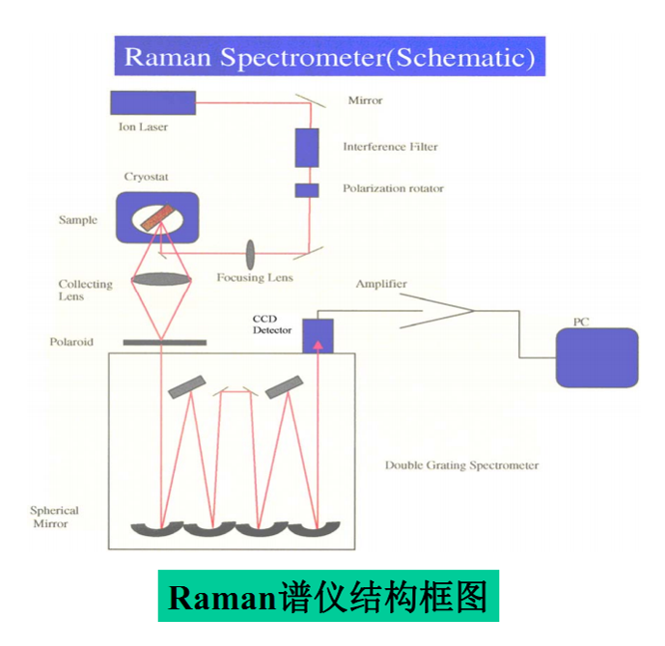
\includegraphics[width = 0.75\linewidth]{Spectrometer_stru.png}
		\paragraph{仪器使用注意事项}
		\begin{enumerate}
			\item	保证使用环境:具备暗室条件;无强震动源、无强电磁干扰;不可受阳光直射。
			\item	光学器件表面有灰尘,不允许接触擦拭,
			可用气球小心吹掉。
			\item	实验结束,首先取出样品进行回收或废弃处理。
			\item	注意激光器电源开、关机的顺序正好相反。
		\end{enumerate}
		\paragraph{实验内容}
		
		1、了解Raman测试系统组成及要求。
		
		2、学习使用拉曼谱仪并测量材料的拉曼光谱。
		
		3、学习处理分析拉曼光谱数据。
		
		
		
		\section{实验数据分析}
		\subsection{测量$CCl_4$分子的拉曼光谱}
		实验测得光谱如图:
		
		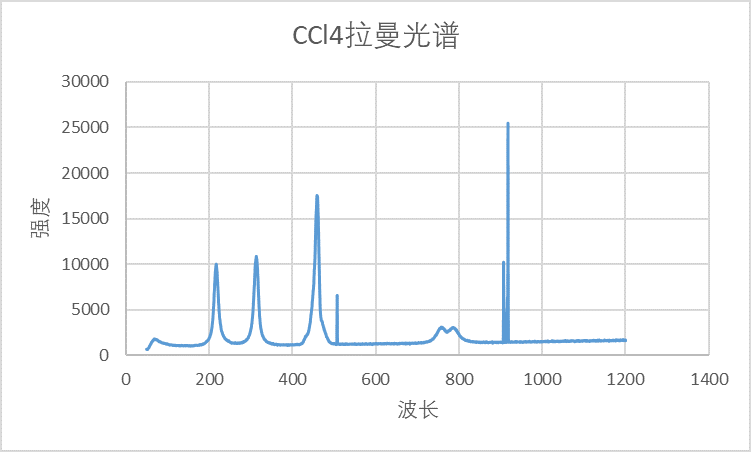
\includegraphics[width = 0.75\linewidth]{Riemann_CCl4.png}
		
		图中有三条尖细的谱线是实验中的噪声,可以忽略不计
		
		\subsection{测量金刚石和碳化硅的拉曼光谱,并通过拉曼光谱区分二者}
		测绘得到的光谱如下:
		
		一号物质:
		
		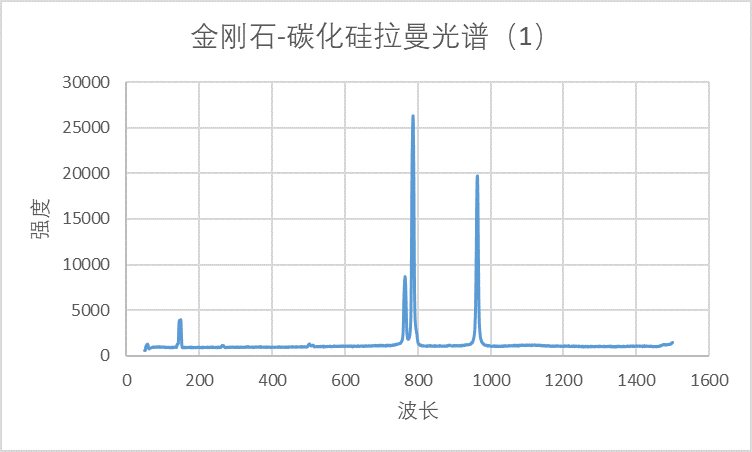
\includegraphics[width = 0.75\linewidth]{Riemann_C_SiC_1.png}
		
		二号物质:
		
		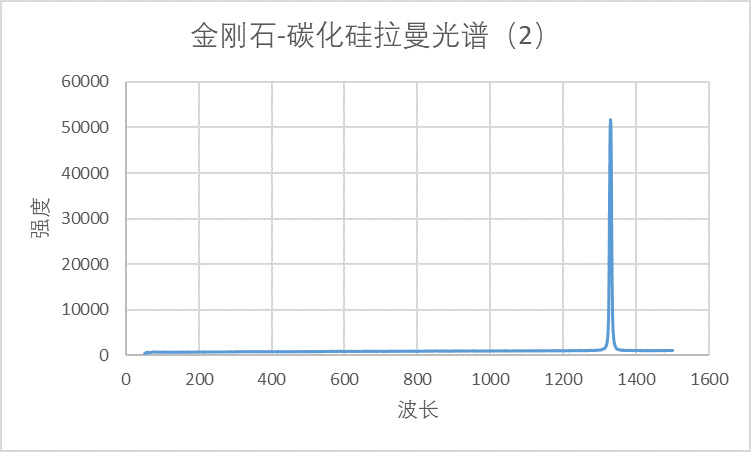
\includegraphics[width = 0.75\linewidth]{Riemann_C_SiC_2.png}
		
		有关文献指出金刚石与碳化硅的拉曼光谱分别为:
		
		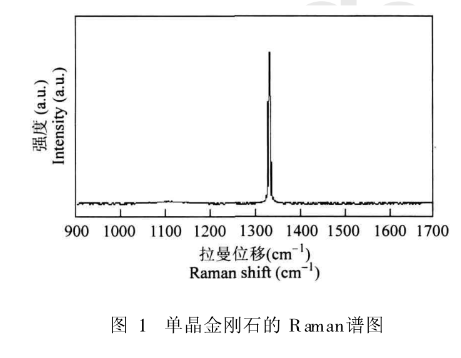
\includegraphics[width = 0.75\linewidth]{Riemann_C.png}
		
		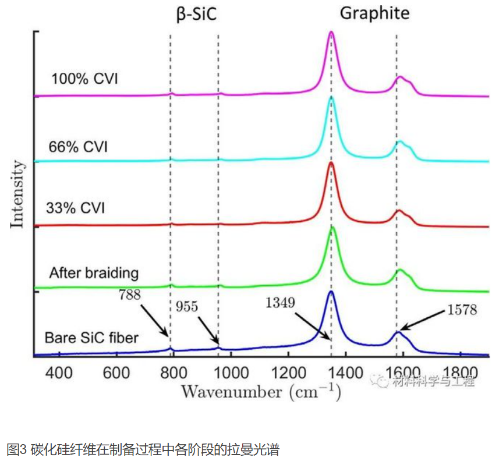
\includegraphics[width = 0.75\linewidth]{Riemann_SiC.png}
		
		将两张图的峰位信息与峰值波长进行对比,我们可以分辨一号物质为碳化硅,二号物质为金刚石。
		
		\section{总结}
		
		本次实验中,我们学习了拉曼光谱仪的有关操作。我们在利用单晶硅矫正仪器的基础上,测量了$CCl_4$的拉曼光谱特征;我们通过测量拉曼光谱,结合有关资料给出的碳化硅与金刚石的光谱,成功区分了这两组物理性质相似的晶体。通过本次实验,我们熟悉了拉曼光谱的特征与如何运用,为以后的生产生活打下坚实基础。
		
		\section{思考题}
		\paragraph{1、本实验所用拉曼光谱仪测试的为stokes部分,如何改变光路设置以能测试anti-stokes部分?}
		
		减小采集的光谱的波长。因为anti-stokes部分频率较高,波长较短。
		
		
		\paragraph{2.在拉曼光谱测量中有哪些可以改变的参数?测试过程中应注意什么?}
		
		样品的浓度,激光功率,以及软件中设置的参数(光谱采集时间等)
		
		
		在测量过程中应该注意防止激光照射眼睛,以及减少对仪器的震动,以及对焦的时候要尽可能让光聚焦在样品的剖面上
		
		
		\paragraph{3. 如何判断测试峰是Raman信号还是荧光信号还是杂散信号?}
		
		如果是荧光信号,则该谱线应该有一定宽度,如果是杂散信号,则该谱线会非常尖细。
		
		\section*{鸣谢}
		感谢中国科学技术大学第一教学楼 物理实验教学中心提供的器材支持与教师指导
		
		
		感谢同学和助教的无私解答与帮助
		
		
		\begin{thebibliography}{100}%此处数字为最多可添加的参考文献数量
			\bibitem{article1}拉曼光谱实验 实验PPT
			
			
			中国科学技术大学物理实验教学中心\quad 著
			
			\bibitem{article2}拉曼光谱实验 实验报告
			
			朱庆庆\quad 著
			
		\end{thebibliography}
		
	\end{multicols}
\end{document}
